\chapter{Modelos De Markov Ocultos}

En este capítulo, estudiaremos un tipo especial de proceso estocástico llamado modelo de Markov oculto (HMM). Empezaremos introduciendo estos modelos, para después seguir discutiendo sobre los problemas y algoritmos que conllevan. En adelante, utilizaremos la abreviatura HMM para referirnos a los modelos de Markov ocultos. 

Este capítulo se basa principalmente en \cite{Rabiner}, \cite[Capítulo 2]{Stamp} y \cite{Jurafsky}.
\section{Extensión a modelos de Markov ocultos }
Hasta ahora hemos considerado cadenas de Markov en las cuales cada estado es un evento observable (o material). Este modelo es demasiado restrictivo para aplicar a numerosos problemas en los que no podemos observar directamente los acontecimientos que nos interesan. Para estudiar este tipo de problema extendemos el concepto de cadena de Markov para incluir los casos en los que la observación es una función probabilística del estado. Como resultado, obtenemos un proceso estocástico conjunto formado por una cadena de Markov homogénea que no es observable (es decir, oculta) pero que produce una serie de consecuencias perceptibles mediante otro proceso estocástico. Es decir, tendremos una cadena $\{\mathcal{X}_t\}_{t=0}^{\infty}$ que representa los sucesos ocultos y un proceso $\{\mathcal{Y}_t\}_{t=0}^{\infty}$ que representa las consecuencias observadas de $\{\mathcal{X}_t\}$. 

Para aclarar esta idea, consideramos el siguiente ejemplo \cite{Russell}:
\begin{exampleth}\label{ejemplo_paraguas}
Un guardia de seguridad trabaja en una instalación subterránea, sin conexión con el exterior. Cada día, no puede saber si está lloviendo o no, pero por las mañanas ve llegar al director con o sin paraguas.

En este caso, $\mathcal{X}_t$ indica si llueve o no en el día $t$ e $\mathcal{Y}_t$ indica si el director lleva o no paraguas. Está claro que $\mathcal{Y}_t$ es consecuencia directa de $\mathcal{X}_t$ y asumiendo que la posibilidad de que llueva en un día determinado depende únicamente del tiempo del día anterior, tenemos que $\{\mathcal{X}_t\}$ es una cadena de Markov homogénea.
\end{exampleth}

Una representación común de la estructura de HMM es la siguiente:
\begin{figure}[H]
\centering

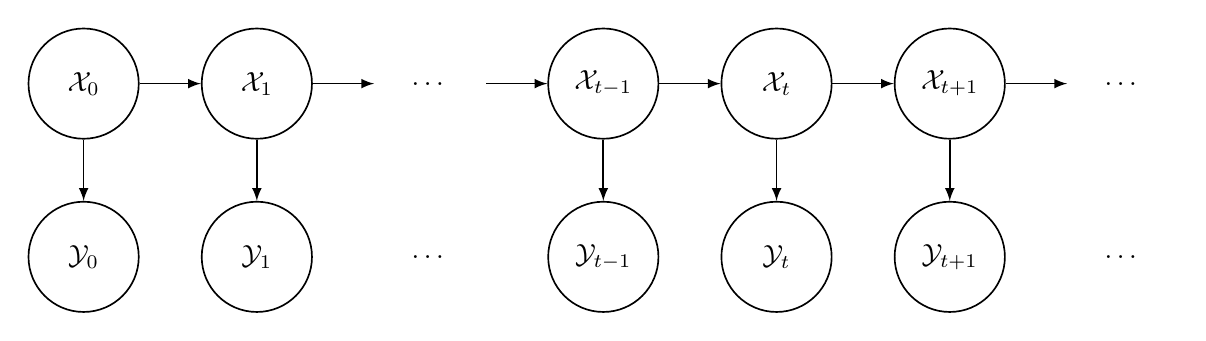
\begin{tikzpicture}[-latex ,auto , node distance =2.2 cm ,semithick,
main/.style = {draw, circle, minimum size=1.4cm}] 
    \node[main] (1) {$\mathcal{X}_0$}; 
    \node[main] (2) [right of=1] {$\mathcal{X}_1$};
    \node[main] (3) [right of=2, draw=none] {\dots};
    \node[main] (4) [right of=3] {$\mathcal{X}_{t-1}$};
    \node[main] (5) [right of=4] {$\mathcal{X}_{t}$};
    \node[main] (6) [right of=5] {$\mathcal{X}_{t+1}$};
    \node[main] (7) [right of=6, draw=none] {\dots};
    
    \node[main] (8) [below of=1] {$\mathcal{Y}_0$}; 
    \node[main] (9) [right of=8] {$\mathcal{Y}_1$};
    \node[main] (10) [right of=9, draw=none] {\dots};
    \node[main] (11) [right of=10] {$\mathcal{Y}_{t-1}$};
    \node[main] (12) [right of=11] {$\mathcal{Y}_{t}$};
    \node[main] (13) [right of=12] {$\mathcal{Y}_{t+1}$};
    \node[main] (14) [right of=13, draw=none] {\dots};

    \draw (1) -- node[midway] {} (2);
    \draw (2) -- node[midway] {} (3);
    \draw (3) -- node[midway] {} (4);
    \draw (4) -- node[midway] {} (5);
    \draw (5) -- node[midway] {} (6);
    \draw (6) -- node[midway] {} (7);
    
    
    \draw (1) -- node[midway] {} (8);
    \draw (2) -- node[midway] {} (9);
    \draw (4) -- node[midway] {} (11);
    \draw (5) -- node[midway] {} (12);
    \draw (6) -- node[midway] {} (13);
    
\end{tikzpicture}
\caption{Estructura de un HMM}
\end{figure}

La representación anterior y el ejemplo \ref{ejemplo_paraguas} nos dan una idea de lo que es un HMM. Para concretarlo, damos la siguiente definición:

\begin{definition}
Sean $\{\mathcal{X}_t\}_{t=0}^{\infty}$ e $\{\mathcal{Y}_t\}_{t=0}^{\infty}$ procesos estocásticos que toman valores en conjuntos finitos $\mathbb{S}=\{s_1,\dots ,s_N\}$ y $\mathbb{V}=\{v_1,\dots ,v_M\}$ respectivamente. El proceso conjunto $\{\left(\mathcal{X}_t,\mathcal{Y}_t\right)\}$ es un modelo de Markov oculto si:
\begin{itemize}
    \item $\{\mathcal{X}_t\}$ es una cadena de Markov homogénea. 
    \item $P[\mathcal{Y}_t=y_t|\mathcal{X}_0=x_0,\dots,\mathcal{X}_t=x_t,\mathcal{Y}_0=y_0,\dots,\mathcal{Y}_{t-1}=y_{t-1}]=P[\mathcal{Y}_t=y_t|\mathcal{X}_t=x_t]$, es decir, la observación en el instante $t$ depende únicamente del estado que se encuentra en dicho momento. Llamaremos a esta probabilidad la probabilidad de emisión.
\end{itemize}

\end{definition}

En distintas fuentes, en lugar de dar una definición explícita de HMM nombran los elementos que lo caracterizan. Puesto que son de enorme importancia, vamos a presentarlos a continuación. Un HMM se caracteriza por:
\begin{enumerate}
\item El conjunto de estados $\mathbb{S}=\{s_1,\dots ,s_N\}$ que, a pesar de no ser observables, suelen conllevar un significado físico del problema.
\item El conjunto de posibles observaciones $\mathbb{V}=\{v_1,\dots ,v_M\}$ que corresponden a las salidas materiales del sistema.
\item La matriz de transición $A$ asociada a $\{\mathcal{X}_t\}$ con:
\[a_{ij} = P[\mathcal{X}_{t+1}=s_j|\mathcal{X}_t=s_i]\]
\item La matriz de emisiones $B\in\left[0,1\right]^{N\times M}$ estocástica con:
\[b_{jk} = P[\mathcal{Y}_{t}=v_k|\mathcal{X}_t=s_j] \text{ para todo $t\geq0$}\]
Para reducir la confusión, en adelante utilizaremos la notación $b_{s_j}(v_k)$ para referirnos a estas probabilidades.
\item Una distribución inicial $\pi\in\Delta^{N-1}$ tal que:
\[P[\mathcal{X}_{0}=s_i]=\pi_i\]
\end{enumerate}

Es frecuente (véase \cite{Rabiner}) utilizar la notación:
\[\lambda=\left(A,B,\pi\right) \tag{3.\arabic{HMM}} \label{notacionHMM}\]
para representar un HMM.

\section{Los tres problemas básicos de los HMMs}
A partir de los conceptos anteriores, podemos identificar 3 entidades: el modelo, la secuencia de observaciones o de salidas y la secuencia de estados. Existen 3 problemas básicos de interés que involucran a estas entidades:
\begin{enumerate}
\item Dado un modelo, ¿cuál es la probabilidad de observar una secuencia particular de salidas? En este caso no nos interesa la secuencia de estados, tan sólo queremos conocer la probabilidad de que ocurran ciertas observaciones.
\item Dado un modelo y una secuencia de salidas, ¿cuál es la secuencia de estados más probable que genera dichas salidas?
\item Dada una secuencia de salidas y conocido el espacio de estados, ¿cuál es el modelo que maximiza la probabilidad de observar dichas salidas?
\end{enumerate}

El \textbf{problema 1} es un problema de evaluación donde calculamos la probabilidad de observar una secuencia de salidas conocido el modelo. También nos permite conocer si el modelo se ajusta a dicha secuencia. Esto puede ser útil, por ejemplo, si estamos considerando varios modelos posibles. En ese caso, la solución del \textbf{problema 1} nos permitiría elegir el modelo que más se ajuste a las observaciones.

En el caso del ejemplo \ref{ejemplo_paraguas}, un ejemplo del \textbf{problema 1} podría ser calcular la probabilidad de que el director lleve paraguas dos días seguidos y no en el tercero.

El \textbf{problema 2} es donde intentamos cubrir la parte oculta del modelo, es decir, encontrar la secuencia \enquote{correcta} de estados. Está claro que en realidad no existe una secuencia \enquote{correcta}. Por ello, utilizaremos criterios de optimalidad para resolver este problema de la mejor manera posible. 

En el caso del ejemplo \ref{ejemplo_paraguas}, si se observa el paraguas en los dos primeros días y no en el tercero, parece lógico pensar que ha llovido en esos dos primeros días y no en el tercero. Veremos que es efectivamente así resolviendo este problema mediante el algoritmo de Viterbi.

En el \textbf{problema 3} pretendemos optimizar los parámetros del modelo dada una secuencia de salidas. La secuencia de observaciones usada para ajustar los parámetros se suele denominar secuencia de entrenamiento. El entrenamiento de HMM es importante, pues así podemos adaptar los parámetros a los datos percibidos. A partir de los resultados, podemos formular mejores modelos para describir fenómenos reales.

Como ejemplo, vamos considerar un problema de reconocimiento de voz, una de las aplicaciones más conocidas de HMM. Podemos utilizar las soluciones del \textbf{problema 3} para entrenar un HMM $\lambda_0$ (usando la notación \eqref{notacionHMM}) que reconoce la pronunciación de la palabra \enquote{no} y otro HMM $\lambda_1$ que reconoce la pronunciación del \enquote{sí}. Entonces dada la pronunciación de una palabra desconocida, podemos calcular la probabilidad de dicha pronunciación en cada uno de los dos modelos usando la solución del \textbf{problema 1}. Así, podemos determinar si la palabra se asemeja más al \enquote{sí} o al \enquote{no}.  

En las siguientes subsecciones vamos a intentar solucionar estos problemas siguiendo principalmente la metodología descrita en \cite{Rabiner}. Notemos que, por ser $\{\mathcal{X}_t\}$ homogénea y por el hecho de que $\mathcal{Y}_t$ depende únicamente del estado en el instante $t$, el instante en el que se comienza a observar las salidas es indiferente. Por lo tanto, podemos suponer siempre que las observaciones inician en el instante $t=0$.

\subsection{Solución al problema 1}
Queremos calcular la probabilidad de una secuencia de observaciones concreta, $O=(O_0,O_1,$ $\dots, O_r)$ conocido el modelo. La forma más directa de hacerlo es mediante enumeración de todas las posibles secuencias de estados de longitud $r+1$. Consideramos una de ellas:
\[Q=(q_0 , q_1 , \dots , q_r)\in\mathbb{S}^{r+1}\]
siendo $q_0$ el estado inicial. Para facilitar la escritura, introducimos la siguiente notación:
\[\mathcal{Y}_k^l:=(\mathcal{Y}_{k},\mathcal{Y}_{k+1},\dots,\mathcal{Y}_{l-1},\mathcal{Y}_{l})\]
Además, dada la secuencia $Q$, para representar las probabilidades de transición a partir de los estados de la secuencia pondremos:
\[a_{q_iq_j}=P[\mathcal{X}_{t+1}=q_j|\mathcal{X}_t=q_i]\]
Usando la notación anterior, la probabilidad de la secuencia de observaciones $O$ dada la secuencia de estados $Q$ es:
\[P[\mathcal{Y}_0^r=O|\mathcal{X}_0^r=Q]=\prod_{t=0}^r P[\mathcal{Y}_{t}=O_t|\mathcal{X}_{t}=q_t]\]
donde aplicamos la independencia entre las observaciones. Por lo tanto:
\[P[\mathcal{Y}_0^r=O|\mathcal{X}_0^r=Q]=b_{q_0}(O_0)\cdot b_{q_1}(O_1)\cdots b_{q_r}(O_r)\]
Y la probabilidad de dicha secuencia de estados $Q$ se puede calcular como:
\[P[\mathcal{X}_0^r=Q]=\pi_{q_0}\cdot a_{q_0q_1}\cdot a_{q_1q_2}\cdots a_{q_{r-1}q_r} \]
Es claro que:
\[P[\mathcal{Y}_0^r=O,\mathcal{X}_0^r=Q]=P[\mathcal{Y}_0^r=O|\mathcal{X}_0^r=Q]\cdot P[\mathcal{X}_0^r=Q] \]
Y la probabilidad de $O$ se puede obtener sumando esta probabilidad mediante todas las posibles secuencias de estados:
\[P[\mathcal{Y}_0^r=O]=\sum_{Q\in\mathbb{S}^{r+1}}P[\mathcal{Y}_0^r=O|\mathcal{X}_0^r=Q]\cdot P[\mathcal{X}_0^r=Q]\]
\[=\sum_{(q_0 , q_1 , \dots , q_r)\in\mathbb{S}^{r+1}}\pi_{q_0}\cdot b_{q_0}(O_0)\cdot a_{q_0q_1}\cdot b_{q_1}(O_1)\cdots a_{q_{r-1}q_r}\cdot b_{q_r}(O_r)\]

Esta manera de calcular, involucra un orden de $2\cdot(r+1)\cdot N^{(r+1)}$ operaciones, puesto que existen $N^{(r+1)}$ posibles secuencias de estados y para cada una de estas secuencias hay que realizar $2\cdot(r+1)$ cálculos. Esto hace imposible calcular esta probabilidad, pues incluso para un modelo de $5$ estados, si se quiere calcular la probabilidad de una secuencia con $100$ observaciones $(r=99)$ se necesitarían $2\cdot100\cdot5^{100}\approx10^{72}$ operaciones. Afortunadamente, existe una forma más eficiente de resolver el \textbf{problema 1} y es mediante el conocido como \textbf{algoritmo de avance-retroceso}. 

\begin{definition}
Definimos la \textbf{variable de avance} $\alpha_t(i)$ como la probabilidad de observar la secuencia parcial $(O_0,O_1,\dots,O_t)$ y que el estado en el instante $t$ sea $s_i$:
\[ \alpha_t(i)=P[\mathcal{Y}_0^t=(O_0,\dots,O_t), \mathcal{X}_t=s_i]\]
\end{definition}
En el instante inicial $t=0$, para todo $i\in\{1,\dots,N\}$:
\[ \alpha_0(i)=P[\mathcal{Y}_0=O_0, \mathcal{X}_0=s_i]=P[\mathcal{Y}_0=O_0|\mathcal{X}_0=s_i]\cdot P[\mathcal{X}_0=s_i]=b_{s_i}(O_0)\cdot\pi_i\]
Suponiendo que conocemos las $\alpha_{t}(i)$ para todo $i$, podemos calcular fácilmente $\alpha_{t+1}(j)$, que es la probabilidad de observar $(O_0,O_1,\dots,O_{t+1})$ y $\mathcal{X}_{t+1}=s_j$. Puesto que queremos que $\mathcal{X}_{t+1}=s_j$, primero calculamos la probabilidad de mantener la secuencia parcial $(O_0,\dots,O_t)$ actualizado el estado, esto no es más que la suma de las variables de avance en $t$ multiplicados por las probabilidades de transición:
\[
\begin{aligned}
    &P[\mathcal{Y}_0^t=(O_0,\dots,O_t), \mathcal{X}_{t+1}=s_j]=\\
    &=\sum_{i=1}^N P[\mathcal{Y}_0^t=(O_0,\dots,O_t), \mathcal{X}_{t}=s_i]\cdot P[\mathcal{X}_{t+1}=s_j|\mathcal{X}_{t}=s_i]\\
    &=\sum_{i=1}^N\alpha_{t}(i)\cdot a_{ij}
\end{aligned}    
\]
Dado que $\mathcal{Y}_{t+1}$ depende únicamente de $\mathcal{X}_{t+1}$, una vez conocida la suma anterior:
\[
\begin{aligned}
    \alpha_{t+1}(j)&=P[\mathcal{Y}_0^{t+1}=(O_0,\dots,O_t,O_{t+1}), \mathcal{X}_{t+1}=s_j]\\
    &=P[\mathcal{Y}_0^t=(O_0,\dots,O_t), \mathcal{X}_{t+1}=s_j]\cdot P[\mathcal{Y}_{t+1}=O_{t+1}|\mathcal{X}_{t+1}=s_j]\\
    &=\left(\sum_{i=1}^N\alpha_{t}(i)\cdot a_{ij}\right)\cdot b_{s_j}(O_{t+1})
\end{aligned}
\]

Luego podemos calcular las variables de avance de forma recursiva:
\begin{equation}
    \alpha_{t+1}(j)=\left(\sum_{i=1}^N\alpha_{t}(i)\cdot a_{ij}\right)\cdot b_{s_j}(O_{t+1}), \qquad 0\leq t\leq r-1 , \quad 1\leq j\leq N \HMMadd \label{fowardRecursivo}
\end{equation}
    
Finalmente, notemos que:
\[
\HMMadd \label{fowardSecuencia}
P[\mathcal{Y}_0^r=O]=\sum_{i=1}^N P[\mathcal{Y}_0^r=O, \mathcal{X}_r=s_i]=\sum_{i=1}^N \alpha_r(i)\]
Si revisamos el cálculo de las variables de avance $\alpha_t(j)$, podemos ver que para cada estado se necesitan $2N$ operaciones en una etapa $t>0$, puesto que hay $N$ estados. Podemos concluir que el cálculo de todas las variables de avance requiere un orden de $2r N^2$ operaciones. Si $N=5$ y $r=99$, necesitaríamos alrededor de $5000$ operaciones usando el algoritmo de avance, en comparación con $10^{72}$ operaciones que requiere el cálculo directo. 

A continuación vamos a utilizar el sencillo caso del ejemplo \ref{ejemplo_paraguas} para poner en práctica lo que acabamos de ver:
\begin{exampleth}[\cite{Sevilla_2019}] \label{ejemplo_paraguasSol1}
En primer lugar vamos a concretar el modelo: representamos el conjunto de estados como $\mathbb{S}=\{R,\neg R\}$ entendiendo $R$ como lluvia. El conjunto de observaciones también tiene cardinalidad $2$: $\mathbb{V}=\{U,\neg U\}$ entendiendo $U$ como presencia de paraguas. Además, vamos a concretar los parámetros del modelo como sigue:
\begin{center}
    $A=\begin{pmatrix}
    0.7 & 0.3\\
    0.3 & 0.7
    \end{pmatrix}$
\end{center}
\begin{center}
    $B=\begin{pmatrix}
    0.9 & 0.1 \\
    0.2 & 0.8
    \end{pmatrix}$
\end{center}
\begin{center}
    $\pi=\begin{pmatrix}
    0.5 & 0.5
    \end{pmatrix}$
\end{center}
Con estos datos, podemos representar el modelo mediante la siguiente gráfica:

\begin{figure}[H]
\centering
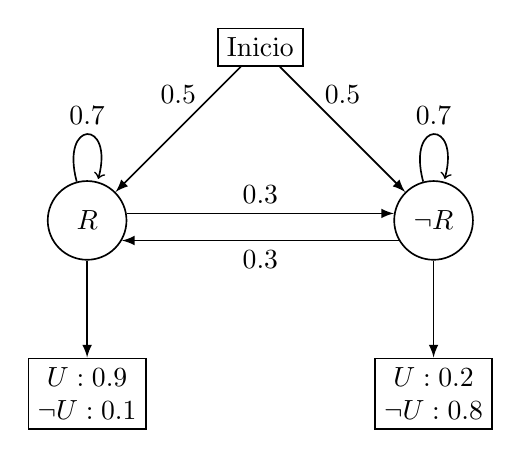
\begin{tikzpicture}[-latex ,auto , node distance =2.2 cm ,semithick, main/.style = {draw, circle, minimum size=1cm}] 
    \node[rectangle, draw, align=center] (1) {Inicio};
    \node[main] (2) [left of=1, below of=1] {$R$};
    \node[main] (3) [right of=1, below of=1] {$\neg R$};
    \node[rectangle, draw, align=center] (4) [below of=2]{$U: 0.9$\\  $\neg U: 0.1$};
    \node[rectangle, draw, align=center] (5) [below of=3]{$U: 0.2$\\  $\neg U: 0.8$};

    \draw (1) -- node[above=0.2cm] {$0.5$} (2);
    \draw (1) -- node[above=0.2cm] {$0.5$} (3);
    \path (2) edge [loop above] node {$0.7$} (2);
    \draw (2.10) -- node[midway] {$0.3$} (3.170);
    \path (3) edge [loop above] node {$0.7$} (3);
    \draw (3. 210) -- node[midway] {$0.3$} (2.330);
    
    \draw (2) -- node[] {} (4);
    \draw (3) -- node[] {} (5);
\end{tikzpicture}
\end{figure}

donde los nodos circulares representan los estados. Los valores de los arcos desde el inicio a los estados corresponden con las probabilidades de la distribución inicial, los valores entre los estados corresponden con las probabilidades de transición y los valores de los recuadros rectangulares corresponden con las probabilidades de emisión desde cada estado.

Volviendo a nuestro ejemplo, supongamos que queremos calcular la probabilidad de observar la secuencia $O=(O_0,O_1,O_2)=(U,U,\neg U)$, calculamos las variables de avance hasta $r=2$ teniendo en cuenta que $s_1=R$ y $s_2=\neg R$:
\begin{itemize}
    \item $t=0$:
    \[\alpha_0(1)=b_{s_1}(O_0)\cdot\pi_1=0.9\cdot0.5=0.45\]
    \[\alpha_0(2)=b_{s_2}(O_0)\cdot\pi_2=0.2\cdot0.5=0.1\]
    \item $t=1$:
    \[
    \begin{aligned}
        \alpha_1(1)&=b_{s_1}(O_1)\cdot\left(\alpha_0(1)\cdot a_{11}+\alpha_0(2)\cdot a_{21} \right)\\
        &=0.9\cdot\left( 0.45\cdot0.7+0.1\cdot0.3 \right) = 0.3105
    \end{aligned}
    \]
    \[
    \begin{aligned}
        \alpha_1(2)&=b_{s_2}(O_1)\cdot\left(\alpha_0(1)\cdot a_{12}+\alpha_0(2)\cdot a_{22} \right)\\
        &=0.2\cdot\left(0.45\cdot0.3+0.1\cdot0.7\right)=0.041
    \end{aligned}
    \]
    \item $t=2$:
    \[
    \begin{aligned}
        \alpha_2(1)&=b_{s_1}(O_2)\cdot\left(\alpha_1(1)\cdot a_{11}+\alpha_1(2)\cdot a_{21} \right)\\
        &=0.1\cdot\left( 0.3105\cdot0.7+0.041\cdot0.3 \right) = 0.022965
    \end{aligned}
    \]
    \[
    \begin{aligned}
        \alpha_2(2)&=b_{s_2}(O_2)\cdot\left(\alpha_1(1)\cdot a_{12}+\alpha_1(2)\cdot a_{22} \right)\\
        &=0.8\cdot\left(0.3105\cdot0.3+0.041\cdot0.7\right)=0.09748
    \end{aligned}
    \]
\end{itemize}
Así, la probabilidad de que el director lleve paraguas dos días seguidos y no en el tercero es:
\[P[\mathcal{Y}_0^2=(U,U,\neg U)]=\alpha_2(1)+\alpha_2(2)=0.022965+0.09748=0.120445\]
\end{exampleth}

La parte de retroceso del algoritmo no es necesaria para resolver \textbf{problema 1}, pero se va a usar en las soluciones a los \textbf{problemas 2 y 3}, así que vamos a presentarla aquí. 

\begin{definition}
Definimos \textbf{la variable de retroceso} $\beta_t(i)$ como la probabilidad de observar la secuencia parcial $(O_{t+1},O_{t+1},\dots,O_{r})$ condicionada a que en el instante $t$, el estado sea $s_i$. Es decir:
\[\beta_t(i)=P[\mathcal{Y}_{t+1}^r=(O_{t+1},O_{t+2},\dots,O_{r})|\mathcal{X}_t=s_i]\]
\end{definition}

Puesto que la secuencia de salidas acaba en $O_r$, $\beta_r(i)$ no se puede determinar usando la definición anterior. En este caso, se define:
\[\beta_r(i)=1, \qquad \forall i\in\{1,\dots,N\}\]
De forma similar a las variables de avance, podemos calcular $\beta_t(i)$ en base a $\beta_{t+1}(j)$. Puesto que conocemos éstos últimos, solo tenemos que preocuparnos por $O_{t+1}$. De nuevo, dado que $\mathcal{Y}_t$ depende únicamente de $\mathcal{X}_t$:
\[
\begin{aligned}
    &P[\mathcal{Y}_{t+1}^r=(O_{t+1},O_{t+2},\dots,O_{r})|\mathcal{X}_{t+1}=s_j]=\\
    &=P[\mathcal{Y}_{t+1}=O_{t+1}|\mathcal{X}_{t+1}=s_j]\cdot P[\mathcal{Y}_{t+2}^r=(O_{t+2},O_{t+3},\dots,O_{r})|\mathcal{X}_{t+1}=s_j]\\
    &=b_{s_j}(O_{t+1})\cdot\beta_{t+1}(j)
\end{aligned}
\]
Además, puesto que $\mathcal{X}_{t+1}$ depende de $\mathcal{X}_t$:
\[
\begin{aligned}
    \beta_t(i)&=P[\mathcal{Y}_{t+1}^r=(O_{t+1},O_{t+2},\dots,O_{r})|\mathcal{X}_t=s_i]\\
    &=\sum_{j=1}^N P[\mathcal{X}_{t+1}=s_j|\mathcal{X}_t=s_i]\cdot P[\mathcal{Y}_{t+1}^r=(O_{t+1},O_{t+2},\dots,O_{r})|\mathcal{X}_{t+1}=s_j]\\
    &=\sum_{j=1}^N a_{ij}\cdot b_{s_j}(O_{t+1})\cdot\beta_{t+1}(j)
\end{aligned}
\]
Luego también podemos calcular las variables de retroceso de forma recursiva:
\begin{equation}
    \beta_t(i)=\sum_{j=1}^N a_{ij}\cdot b_{s_j}(O_{t+1})\cdot\beta_{t+1}(j), \qquad 0\leq t\leq r-1, \quad 1\leq i\leq N \HMMadd \label{backwardRecursivo}
\end{equation}
Para cada estado, se necesitan $3N-1$ operaciones en una etapa con $0\leq t\leq r-1$. Dado que existen $N$ estados, se requiere un orden de $3r N^2$ operaciones para calcular todas las variables de retroceso.

Veremos en los siguientes apartados, que las variables de avance y de retroceso se usarán para resolver los \textbf{problemas 2 y 3}.

\subsection{Solución al problema 2}
Existen varias formas de resolver el \textbf{problema 2} en el que, a diferencia del \textbf{problema 1}, no es posible dar una solución exacta. Se trata ahora de encontrar una secuencia de estados \enquote{óptima} dada una secuencia de observaciones y un determinado modelo. En primer lugar, debemos definir lo que es una secuencia de estados óptima. Existen varios criterios de optimalidad, uno de ellos consiste en escoger estados que son más probables individualmente. Con este criterio se pretende maximizar el número estimado de estados individuales correctos. Para implementar esta solución al \textbf{problema 2}, definimos la siguiente variable: 
\[\gamma_t(i)=P[\mathcal{X}_t=s_i|\mathcal{Y}_0^r=(O_0,O_1,\dots, O_r)]\]
que es la probabilidad de que el estado en el instante $t$ sea $s_i$ condicionada a observar la secuencia de salidas completa $O=(O_0,O_1,\dots, O_r)$.

\begin{proposition}
$\gamma_t(i)$ se puede expresar en función de las variables de avance y de retroceso de la siguiente forma:
\[\gamma_t(i)=\dfrac{\alpha_t(i)\cdot\beta_t(i)}{\sum\limits_{j=1}\limits^N \alpha_t(j)\cdot\beta_t(j)}\]
\end{proposition}
\begin{proofs*}
Por definición de las variables:
\[
\begin{aligned}
    \alpha_t(i)\cdot\beta_t(i)&=P[\mathcal{Y}_0^t=(O_0,\dots,O_t), \mathcal{X}_t=s_i]\cdot P[\mathcal{Y}_{t+1}^r=(O_{t+1},O_{t+2},\dots,O_{r})|\mathcal{X}_t=s_i]\\
    &=P[\mathcal{Y}_0^r=(O_0,O_1,\dots, O_r),\mathcal{X}_t=s_i]
\end{aligned}
\]
Por lo tanto:
\[
\begin{aligned}
    \dfrac{\alpha_t(i)\cdot\beta_t(i)}{\sum\limits_{j=1}\limits^N \alpha_t(j)\cdot\beta_t(j)}&=\dfrac{P[\mathcal{Y}_0^r=(O_0,O_1,\dots, O_r),\mathcal{X}_t=s_i]}{\sum\limits_{j=1}\limits^N P[\mathcal{Y}_0^r=(O_0,O_1,\dots, O_r),\mathcal{X}_t=s_j]}\\
    &=\dfrac{P[\mathcal{Y}_0^r=(O_0,O_1,\dots, O_r),\mathcal{X}_t=s_i]}{P[\mathcal{Y}_0^r=(O_0,O_1,\dots, O_r)]}
\end{aligned}
\]
Aplicando la definición de probabilidad condicionada tenemos la igualdad del enunciado. \qed 
\end{proofs*}

Usando estas variables, podemos definir los estados más probables individualmente dada la secuencia de observaciones $O$:
\begin{definition}
Sea la secuencia de observaciones $O=(O_0,O_1,\dots,O_r)$, definimos el estado más probable individualmente en el instante $t$ como:
\[
\HMMadd \label{estadoProbableIndividualmente}
q_t=\argmax_{1\leq i\leq N}\{\gamma_t(i)\}=\{s_i\in\mathbb{S}\,|\,\forall s_j\in\mathbb{S}:\gamma_t(j)\leq\gamma_t(i)\}\]
\end{definition}

A pesar de que \eqref{estadoProbableIndividualmente} maximiza el número estimado de estados correctos, puede haber problemas con la secuencia de estados resultante. Por ejemplo, si existen estados inalcanzables desde una de ellas, la secuencia de estados \enquote{óptima} puede ser inválida. Esto se debe a que la solución proporcionada por \eqref{estadoProbableIndividualmente} sólo determina los estados más probables en cada instante, sin tener en cuenta la probabilidad de existencia de la secuencia resultante en ningún momento. 

Una posible solución a este problema consiste en modificar el criterio. Se pueden considerar secuencias de estados que maximizan el número estimado de parejas $(q_t,q_{t+1})$ o de ternas $(q_t,q_{t+1},q_{t+2})$ de estados correctas. Estos criterios pueden ser razonables para ciertas aplicaciones concretas, pero el criterio más utilizado es el de encontrar la secuencia $Q=(q_0, q_1, \dots, q_r)$ que maximiza $P[\mathcal{X}_0^r=Q|\mathcal{Y}_0^r=O]$. Lo cual es equivalente a maximizar $P[\mathcal{X}_0^r=Q,\mathcal{Y}_0^r=O]$.

Una técnica formal para encontrar dicha secuencia $Q$ existe, se basa en métodos de programación dinámica y se llama \textbf{algoritmo de Viterbi}. En primer lugar definimos la variable de Viterbi:
\[
\begin{aligned}
    \delta_t(i):&=\max_{(q_0,q_1\dots,q_{t-1})\in\mathbb{S}^t}P[\mathcal{X}_0^{t-1}=(q_0,q_1,\dots,q_{t-1}),\mathcal{X}_t=s_i,\mathcal{Y}_0^t=(O_0,\dots,O_t)]\\
    &=\max_{(q_0,q_1\dots,q_{t-1})\in\mathbb{S}^t}P[\mathcal{X}_0^{t}=(q_0,q_1,\dots,q_{t-1},s_i),\mathcal{Y}_0^t=(O_0,\dots,O_t)]
\end{aligned}
\]

En cada instante, $\delta_t(i)$ nos proporciona la probabilidad de la secuencia de estados más probable $(q_0,q_1,\dots,q_{t-1},q_t)$ de longitud $t+1$ con $q_t=s_i$, habiendo además observado $(O_0,\dots,O_t)$. 

En el instante inicial $t=0$, para todo $i\in\{1,\dots,N\}$:
\[
\begin{aligned}
    \delta_0(i)=P[\mathcal{X}_0=s_i,\mathcal{Y}_0=O_0]=P[\mathcal{X}_0=s_i]\cdot P[\mathcal{Y}_0=O_0|\mathcal{X}_0=s_i]=b_{s_i}(O_0)\cdot\pi_i
\end{aligned}
\]

Notemos que cada $\delta_t(i)$ con $t>0$ se puede calcular recursivamente en función de $\delta_{t-1}(j),1\leq j\leq N$. La idea de la recursividad se debe a la propiedad de Markov, pues la secuencia más probable de estados hasta llegar a $\mathcal{X}_t=s_i$ está compuesta por la secuencia más probable $(q_0,q_1\dots,q_{t-1})$ con $q_{t-1}$ igual a un cierto estado $s_j$ y la transición de $s_j$ a $s_i$. Esta idea se puede observar con la Figura \ref{fig:Viterbi}. 

\begin{figure}[H]
    \centering
    \begin{tikzpicture}[-latex ,auto , node distance = 1.3cm,
    main/.style = {draw, circle, minimum size=0.9cm}, dissapear/.style={draw=none}] 
        \node[main] (1) {$s_1$}; 
        \node[main] (2) [below of=1] {$s_2$};
        \node[main] (3) [below of=2] {$s_3$};
        \node[dissapear] (4) [below = 0mm of 3] {\rvdots};
        \node[main] (5) [below = 0mm of 4] {$s_j$};
        \node[dissapear] (6) [below = 0mm of 5] {\rvdots};
        \node[main] (7) [below = 0mm of 6] {$s_N$};
        
  
        \node[main] (8) [right= 2cm of 1]{$s_1$}; 
        \node[main] (9) [below of=8] {$s_2$};
        \node[main] (10) [below of=9] {$s_3$};
        \node[dissapear] (11) [below= 0mm of 10] {\rvdots};
        \node[main] (12) [below = 0mm of 11] {$s_j$};
        \node[dissapear] (13) [below = 0mm of 12] {\rvdots};
        \node[main] (14) [below = 0mm of 13] {$s_N$};

        \node[dissapear] (15) [right = 1cm of 8]{$\cdots$}; 
        \node[dissapear] (16) [below of=15] {$\cdots$};
        \node[dissapear] (17) [below of=16] {$\cdots$};
        \node[dissapear] (18) [below of=17] {$\cdots$};
        \node[dissapear] (19) [below of= 18] {$\cdots$};

        \node[main] (20) [right = 1cm of 15]{$s_1$}; 
        \node[main] (21) [below of=20] {$s_2$};
        \node[main] (22) [below of=21] {$s_3$};
        \node[dissapear] (23) [below= 0mm of 22] {\rvdots};
        \node[main] (24) [below = 0mm of 23] {$s_j$};
        \node[dissapear] (25) [below = 0mm of 24] {\rvdots};
        \node[main] (26) [below = 0mm of 25] {$s_N$};

        \node[main] (27) [right=2cm of 22]{$s_i$}; 
        \node[dissapear]  (28) [below of =7]{$\mathcal{X}_0$};
        \node[dissapear]  (29) [below of =14]{$\mathcal{X}_1$};
        \node[dissapear]  (30) [below of =26]{$\mathcal{X}_{t-1}$};
        \node[dissapear]  (31) [right = 2 of 30]{$\mathcal{X}_t$};

        \draw [-, ultra thick, cyan] (1) -- (14);
        \draw [-, ultra thick, cyan] (2) -- (9);
        \draw [-, ultra thick, blue] (3) -- (8);
        \draw [-, ultra thick, cyan] (5) -- (10);
        \draw [-, ultra thick, cyan] (7) -- (12);

        \draw [-, ultra thick, blue] (8) -- (17);
        \draw [-, ultra thick, cyan] (9) -- (15);
        \draw [-, ultra thick, cyan] (10) -- (19);
        \draw [-, ultra thick, cyan] (12) -- (18);
        \draw [-, ultra thick, cyan] (14) -- (16);

        \draw [-, ultra thick, blue] (17) -- (24);
        \draw [-, ultra thick, cyan] (15) -- (20);
        \draw [-, ultra thick, cyan] (19) -- (26);
        \draw [-, ultra thick, cyan] (18) -- (21);
        \draw [-, ultra thick, cyan] (16) -- (22);

        \draw [-, ultra thick, pink] (20) -- (27);
        \draw [-, ultra thick, pink] (21) -- (27);
        \draw [-, ultra thick, pink] (22) -- (27);
        \draw [-, ultra thick, red] (24) -- (27);
        \draw [-, ultra thick, pink] (26) -- (27);
    \end{tikzpicture}
    \caption{Recursión de algoritmo de Viterbi \cite{Sevilla_2019}}
    \label{fig:Viterbi}
\end{figure}

Por lo tanto, tenemos que hallar las secuencias más probables hasta $t-1$ y ver desde cuál se obtiene la probabilidad máxima dando un paso más: 

\[
\begin{aligned}
    \delta_t(i)&=\max_{(q_0,\dots,q_{t-1})\in\mathbb{S}^t}P[\mathcal{X}_0^{t-1}=(q_0,\dots,q_{t-1}),\mathcal{X}_t=s_i,\mathcal{Y}_0^t=(O_0,\dots,O_t)]\\
    &=\max_{(q_0,\dots,q_{t-1})\in\mathbb{S}^t}\bigl(P[\mathcal{X}_0^{t-1}=(q_0,\dots,q_{t-1}),\mathcal{X}_t=s_i,\mathcal{Y}_0^{t-1}=(O_0,\dots,O_{t-1})]\\
    &\qquad\cdot P[\mathcal{Y}_t=O_t|\mathcal{X}_0^{t-1}=(q_0,\dots,q_{t-1}),\mathcal{X}_t=s_i,\mathcal{Y}_0^{t-1}=(O_0,\dots,O_{t-1})]\bigr)
\end{aligned}    
\]
Aplicando que $\mathcal{Y}_t$ depende únicamente de $\mathcal{X}_t$:
\[
\begin{aligned}
    \delta_t(i)&=\max_{(q_0,\dots,q_{t-1})\in\mathbb{S}^t}P[\mathcal{X}_0^{t-1}=(q_0,\dots,q_{t-1}),\mathcal{X}_t=s_i,\mathcal{Y}_0^{t-1}=(O_0,\dots,O_{t-1})]\\
    &\qquad\cdot P[\mathcal{Y}_t=O_t|\mathcal{X}_t=s_i]
\end{aligned}    
\]
Utilizando la idea de recursión:
\[
\begin{aligned}
    &\max_{(q_0,\dots,q_{t-1})\in\mathbb{S}^t}P[\mathcal{X}_0^{t-1}=(q_0,\dots,q_{t-1}),\mathcal{X}_t=s_i,\mathcal{Y}_0^{t-1}=(O_0,\dots,O_{t-1})]\\
    &=\max_{j=1,\dots,N}\bigl(P[\mathcal{X}_t=s_i|\mathcal{X}_{t-1}=s_j]\cdot\max_{(q_0,\dots,q_{t-2})\in\mathbb{S}^t}P[\mathcal{X}_0^{t-2}=(q_0,\dots,q_{t-2}),\\
    &\qquad\mathcal{X}_{t-1}=s_j,\mathcal{Y}_0^{t-1}=(O_0,\dots,O_{t-1})]\bigr)\\
    &=\max_{j=1,\dots,N}\left(a_{ji}\cdot\delta_{t-1}(j)\right)
\end{aligned}    
\]
Por lo tanto:
\[\HMMadd \label{formulaDeltaViterbi}
\delta_t(i)= \max_{j=1,\dots,N}\left(a_{ji}\cdot\delta_{t-1}(j)\right) \cdot b_{s_i}(O_t)   
\]

Además, necesitamos tener constancia de los estados que forman parte de la secuencia óptima. Para ello, definimos $\psi_t(i)$ como el estado en el instante $t-1$ que maximiza $\delta_t(i)$. Resumiendo:
\begin{itemize}
    \item En el instante inicial:
    \begin{equation*}
        \delta_0(i)=b_{s_i}(O_0)\cdot\pi_i, \qquad 1\leq i\leq N.
    \end{equation*}
    \item Aplicando recursión:
    \begin{align*}
        &\delta_t(i)=\max_{j=1,\dots,N}\left(a_{ji}\cdot\delta_{t-1}(j)\right) \cdot b_{s_i}(O_t), && 1\leq t\leq r, \\
        &\psi_t(i)=\argmax_{j=1,\dots,N}\left(a_{ji}\cdot\delta_{t-1}(j)\right),  &&  1\leq i\leq N.
    \end{align*}
    \item Finalmente:
    \begin{align*}
        & P^* = \max_{i=1,\dots,N} \delta_r(i)\\
        & q_r^*=\argmax_{i=1,\dots,N} \delta_r(i)
    \end{align*} 
    \item Para encontrar la secuencia de estados óptima:
    \[q_t^*=\psi_{t+1}(q_{t+1}^*), \quad t=r-1,r-2,\dots,0\]
\end{itemize}
Notemos que el esquema recursivo del algoritmo de Viterbi es similar al del algoritmo de avance. La mayor diferencia se encuentra en que, en este caso, se toma el máximo en lugar de calcular una sumatoria.

\begin{exampleth}[\cite{Sevilla_2019}]
Bajo los parámetros del ejemplo \ref{ejemplo_paraguasSol1}, ahora podemos hallar la secuencia de estados más probable habiendo observado el director con paraguas en los dos primeros días y no en el tercero. Recordemos que $O=(O_0,O_1,O_2)=(U,U,\neg U)$ y los estados son $s_1=L$ y $s_2=\neg L$:
\begin{itemize}
    \item $t=0$:
    \[\delta_0(1)=b_{s_1}(O_0)\cdot\pi_1=0.9\cdot0.5=0.45\]
    
    \[\delta_0(2)=b_{s_2}(O_0)\cdot\pi_2=0.2\cdot0.5=0.1\]
    
    \item $t=1$:
    \[\begin{aligned}
        \delta_1(1)&=b_{s_1}(O_1)\cdot\max\{a_{11}\cdot\delta_0(1),\,a_{21}\cdot\delta_0(2)\}\\
        &=0.9\cdot\max\{(0.7\cdot0.45),\,(0.3\cdot0.1)\}\\
        &=0.9\cdot\max\{\underline{0.315},0.03\}=0.2835\\
        \psi_1(1)&=L
    \end{aligned}\]
    
    \[\begin{aligned}
        \delta_1(2)&=b_{s_2}(O_1)\cdot\max\{a_{12}\cdot\delta_0(1),\,a_{22}\cdot\delta_0(2)\}\\
        &=0.2\cdot\max\{(0.3\cdot0.45),\,(0.7\cdot0.1)\}\\
        &=0.2\cdot\max\{\underline{0.135},0.07\}=0.027\\
        \psi_1(2)&=L
    \end{aligned}\]
    
    \item $t=2$:
    \[\begin{aligned}
        \delta_2(1)&=b_{s_1}(O_2)\cdot\max\{a_{11}\cdot\delta_1(1),\,a_{21}\cdot\delta_1(2)\}\\
        &=0.1\cdot\max\{(0.7\cdot0.2835),\,(0.3\cdot0.027)\}\\
        &=0.1\cdot\max\{\underline{0.19845},0.0081\}=0.019845\\
        \psi_2(1)&=L
    \end{aligned}\]
    
    \[\begin{aligned}
        \delta_2(2)&=b_{s_2}(O_2)\cdot\max\{a_{12}\cdot\delta_1(1),\,a_{22}\cdot\delta_1(2)\}\\
        &=0.8\cdot\max\{(0.3\cdot0.2835),\,(0.7\cdot0.027)\}\\
        &=0.8\cdot\max\{\underline{0.08505},0.0189\}=0.06804\\
        \psi_2(2)&=L
    \end{aligned}\]
\end{itemize}
Puesto que $\delta_2(2)>\delta_2(1)$, tomamos $q_2^*=s_2=\neg L$, reconstruyendo la secuencia tenemos que:
\[q_1^*=\psi_2(2)=L=s_1, \quad q_0^*=\psi_1(1)=L\]
Luego la secuencia de estados resultante de aplicar el algoritmo de Viterbi es $Q=(L,L,\neg L)$, lo cual coincide con nuestra intuición.

\end{exampleth}


\subsection{Solución al problema 3}
El tercer problema, y el más complicado, consiste en tratar de determinar un método para ajustar los parámetros del modelo de manera que se maximice la probabilidad de una secuencia de observaciones dada. 

Sin embargo, no existe ninguna forma analítica de resolver este problema de optimización. Dada una secuencia finita de observaciones $O=(O_0,\dots,O_r)$, no existe una manera óptima de estimar los parámetros del modelo.

No obstante, podemos elegir $\lambda=(A,B,\pi)$ de forma que, con estos parámetros, $P[\mathcal{Y}_0^r=O]$ se maximice de forma local. Para determinar estos parámetros vamos a utilizar un algoritmo llamado \textbf{algoritmo de Baum-Welch}. En primer lugar, dado un par de estados $s_i,s_j\in\mathbb{S}$, definimos:
\[\xi_t(i,j):=P[\mathcal{X}_t=s_i,\mathcal{X}_{t+1}=s_j|\mathcal{Y}_{0}^r=O],\qquad 0\leq t\leq r-1\]
que es la probabilidad de que los estados en los instantes $t$ y $t+1$ sean $s_i$ y $s_j$ respectivamente, condicionada a observar la secuencia de salidas completa $O=(O_0,O_1,\dots, O_r)$.
\begin{proposition} 
$\xi_t(i,j)$ se puede expresar en función de las variables de avance y de retroceso de la siguiente forma:
\[
\xi_t(i,j)=\frac{\alpha_t(i)\cdot a_{ij}\cdot b_{s_j}(O_{t+1})\cdot\beta_{t+1}(j)}{\displaystyle\sum_{i=1}^N\sum_{j=1}^N\alpha_t(i)\cdot a_{ij}\cdot b_{s_j}(O_{t+1})\cdot\beta_{t+1}(j) \HMMadd \label{definicionXi}}
\]
\end{proposition}
\begin{proofs*}
Aplicando la definición de probabilidad condicionada:
\[\xi_t(i,j)=\frac{P[\mathcal{X}_t=s_i,\mathcal{X}_{t+1}=s_j,\mathcal{Y}_0^r=O]}{P[\mathcal{Y}_0^r=O]}\]
Veamos que los numeradores coinciden. Por definiciones de las variables de avance y de retroceso:
\[
\begin{aligned}
    \alpha_t(i)\cdot a_{ij}\cdot b_{s_j}(O_{t+1})\cdot\beta_{t+1}(j)&=P[\mathcal{Y}_0^t=(O_0,\dots,O_t),\mathcal{X}_t=s_i]\cdot P[\mathcal{X}_{t+1}=s_j|\mathcal{X}_t=s_i]\\
    &\quad\cdot P[\mathcal{Y}_{t+1}=O_{t+1}|\mathcal{X}_{t+1}=s_j]\\
    &\quad\cdot P[\mathcal{Y}_{t+2}^r=(O_{t+2},\dots,O_r)|\mathcal{X}_{t+1}=s_j]\\
    &=P[\mathcal{Y}_0^t=(O_0,\dots,O_t),\mathcal{X}_t=s_i,\mathcal{X}_{t+1}=s_j,\\
    &\qquad\mathcal{Y}_{t+1}=O_{t+1},\mathcal{Y}_{t+2}^r=(O_{t+2},\dots,O_r)]\\
    &=P[\mathcal{Y}_0^r=(O_0,\dots,O_r),\mathcal{X}_t=s_i,\mathcal{X}_{t+1}=s_j]
\end{aligned}
\]
Teniendo esto, podemos ver que los denominadores también coinciden:
\begin{align*}
    P[\mathcal{Y}_{0}^r=O]&= \sum_{i=1}^N\sum_{j=1}^N P[\mathcal{Y}_0^r=O,\mathcal{X}_t=s_i,\mathcal{X}_{t+1}=s_j]\\
    &=\sum_{i=1}^N\sum_{j=1}^N\alpha_t(i)\cdot a_{ij}\cdot b_{s_j}(O_{t+1})\cdot\beta_{t+1}(j) \tag*{\qedsymbol}
\end{align*}

\end{proofs*}

Recordemos que previamente habíamos definido la variable $\gamma_t(i)$ como:
\[\gamma_t(i)=P[\mathcal{X}_t=s_i|\mathcal{Y}_0^r=O]\]

No es difícil ver a partir de las definiciones, que:
\[\gamma_t(i)=\sum_{j=1}^N\xi_t(i,j), \qquad 0\leq t\leq r-1\]

Si sumamos $\gamma_t(i)$ con $t$ desde $0$ hasta $r$, obtenemos una cantidad que se puede interpretar como la cantidad esperada de visitas al estado $s_i$. Si excluimos $t=r$, se puede interpretar como el número esperado de transiciones que se realizan a partir de $s_i$. De forma similar, la suma de $\xi_t(i,j)$ con $t$ de $0$ a $r-1$ se puede interpretar como el número esperado de transiciones de $s_i$ a $s_j$. En resumen:
\[\sum_{t=0}^{r}\gamma_t(i)=\text{número esperado de visitas a $s_i$ }\]
\[\sum_{t=0}^{r-1}\gamma_t(i)=\text{número esperado de transiciones desde } s_i\]
\[\sum_{t=0}^{r-1}\xi_t(i,j)=\text{número esperado de transiciones de } s_i \text{ a } s_j\]

Usando lo anterior, podemos dar un método razonable para reestimar los parámetros de un HMM. Definimos:
\[\overline{\pi}_i=\gamma_0(i)=P[\mathcal{X}_0=s_i|\mathcal{Y}_0^r=O]\]
\begin{align*}
    \overline{a}_{ij}&=\dfrac{\text{número esperado de transiciones de $s_i$ a $s_j$}}{\text{número esperado de transiciones desde $s_i$}} \\
    &=\dfrac{\displaystyle\sum_{t=0}^{r-1}\xi_t(i,j)}{\displaystyle\sum_{t=0}^{r-1}\gamma_t(i)}
\end{align*}
\begin{align*}
    \overline{b}_j(k)&=\dfrac{\text{número esperado de visitas a $s_j$ habiendo observado $v_k$}}{\text{número esperado de visitas a $s_j$}}\\
    &=\dfrac{\displaystyle\sum_{\substack{t=0 \\ O_t=v_k}}^{r}\gamma_t(j)}{\displaystyle\sum_{t=0}^{r}\gamma_t(j)}
\end{align*}

Si definimos el modelo actual como $\lambda=(A,B,\pi)$, y lo utilizamos para calcular los parámetros anteriores, podemos definir un modelo reestimado $\overline{\lambda}=(\overline{A},\overline{B},\overline{\pi})$. Entonces está probado que puede ocurrir una de las siguientes opciones \cite{Rabiner}:
\begin{itemize}
    \item el modelo inicial $\lambda$ es un punto crítico de la función de probabilidad, en ese caso $\overline{\lambda}=\lambda$.
    \item la probabilidad de observar la secuencia de salidas $O$ bajo el modelo $\overline{\lambda}$ es mayor que bajo $\lambda$. Es decir, $P[\mathcal{Y}_0^r=O|\overline{\lambda}]>P[\mathcal{Y}_0^r=O|\lambda]$.
\end{itemize}

Con el proceso anterior, podemos iterar reemplazando $\overline{\lambda}$ por $\lambda$. De esta forma, podemos aumentar la probabilidad de observar $O$ hasta llegar a un valor límite. Cabe destacar que este algoritmo es susceptible de caer en un máximo local y en diversos problemas de interés, pueden existir varios máximos locales.

Recordemos que el algoritmo de Baum-Welch se utiliza para reestimar los parámetros de $\lambda=(A,B,\pi)$ con la intención de maximizar $P[\mathcal{Y}_0^r=O|\lambda]$ con $O=(O_0,\cdots,O_r)$ una secuencia de observaciones conocida. Pero también podemos usarlo para determinar los estados de un espacio $\mathbb{S}$ al que sólo se conoce la cardinalidad del espacio: ante problemas en los que no tenemos suficiente información, podemos partir de un modelo inicial estimado y aplicar el algoritmo de Baum-Welch para construir un modelo ajustado mediante una secuencia de observaciones suficientemente amplia. A partir de los resultados, podemos dar un significado físico a los estados del espacio $\mathbb{S}$. Como ejemplo, examinamos el siguiente caso: 


\begin{exampleth}
Consideramos el ejemplo ilustrado en \cite{Stamp}, en el que se pretende estudiar las propiedades básicas del inglés. Para ello, toma el libro \enquote{Brown Corpus} con alrededor de un millón de palabras, eliminó las puntuaciones, números y caracteres especiales y convirtió todas las letras a minúscula obteniendo $26$ posibles letras y el espacio, un total de $27$ símbolos que consideró como posibles observaciones.

Con estas $27$ posibles observaciones y considerando un espacio de estados $\mathbb{S}$ con cardinalidad $N=2$, toma las primeras las primeras $50000$ observaciones y supone que todas las probabilidades se distribuyen de forma aleatoriamente uniforme. En especial, asigna a cada probabilidad de emisión un valor aleatorio cercano a $1/27$. Aplicando $100$ veces el algoritmo de Baum-Welch obtuvo las siguiente probabilidades de emisión:  

%Tomando espacios de estados $\mathbb{S}$ de cardinalidad $N=2,\dots,12$ sin especificar los significados de los estados, la aplicación del algoritmo de Baum-Welch les ha permitido llegar a conclusiones dependiendo de $N$. En particular, para $N=2$ obtuvieron las siguientes probabilidades de observar cada letra estando en uno de los dos estados:

\begin{longtable}{|c|C|C|C|C|}
        \hline
        & \multicolumn{2}{|C|}{\text{Inicial}} & \multicolumn{2}{|C|}{\text{Final}} \\
        \hline
        & s_1 & s_2  & s_1 & s_2 \\
        \hline
        a & 0.03735 & 0.03909 & 0.13845 & 0.00075\\
        \hline
        b & 0.03408 & 0.03537 & 0.00000 & 0.02311\\
        \hline
        c & 0.03455 & 0.03537 & 0.00062 & 0.05614\\
        \hline
        d & 0.03828 & 0.03909 & 0.00000 & 0.06937\\
        \hline
        e & 0.03782 & 0.03583 & 0.21404 & 0.00000\\
        \hline
        f & 0.03922 & 0.03630 & 0.00000 & 0.03559\\
        \hline
        g & 0.03688 & 0.04048 & 0.00081 & 0.02724\\
        \hline
        h & 0.03408 & 0.03537 & 0.00066 & 0.07278\\
        \hline
        i & 0.03875 & 0.03816 & 0.12275 & 0.00000\\
        \hline
        j & 0.04062 & 0.03909 & 0.00000 & 0.00365\\
        \hline
        k & 0.03735 & 0.03490 & 0.00182 & 0.00703\\
        \hline
        l & 0.03968 & 0.03723 & 0.00049 & 0.07231\\
        \hline
        m & 0.03548 & 0.03537 & 0.00000 & 0.03889\\
        \hline
        n & 0.03735 & 0.03909 & 0.00000 & 0.11461\\
        \hline
        o & 0.04062 & 0.03397 & 0.13156 & 0.00000\\
        \hline
        p & 0.03595 & 0.03397 & 0.00040 & 0.03674\\
        \hline
        q & 0.03641 & 0.03816 & 0.00000 & 0.00153\\
        \hline
        r & 0.03408 & 0.03676 & 0.00000 & 0.10225\\
        \hline
        s & 0.04062 & 0.04048 & 0.00000 & 0.11042\\
        \hline
        t & 0.03548 & 0.03443 & 0.01102 & 0.14392\\
        \hline
        u & 0.03922 & 0.03537 & 0.04508 & 0.00000\\
        \hline
        v & 0.04062 & 0.03955 & 0.00000 & 0.01621\\
        \hline
        w & 0.03455 & 0.03816 & 0.00000 & 0.02303\\
        \hline
        x & 0.03595 & 0.03723 & 0.00000 & 0.00447\\
        \hline
        y & 0.03408 & 0.03769 & 0.00019 & 0.02587\\
        \hline
        z & 0.03408 & 0.03955 & 0.00000 & 0.00110\\
        \hline
        espacio &  0.03688 & 0.03397 & 0.33211 &  0.01298\\
        \hline
        \caption{Probabilidades de emisión antes y después de aplicar el algoritmo de Baum-Welch \cite{Stamp}}
\end{longtable}
Si analizamos estas probabilidades, podemos ver que los estados separan las vocales de las consonantes, de forma que $s_1$ representa el conjunto de vocales y $s_2$ representa el conjunto de consonantes.

Este resultado también se ha alcanzado utilizando la traducción del Quijote a inglés \cite{AnálisisVoynich} y no debería de sorprender a una persona que tenga conocimiento sobre el idioma. Sin embargo, permite a personas que carecen de ese conocimiento llegar a conclusiones analizando los resultados obtenidos de un HMM asociado al problema.
\end{exampleth}

\section{Mejora de las soluciones}
No es difícil darse cuenta de que las variables $\alpha_t(i), \beta_t(i)$ y $\delta_t(i)$ tienden a $0$ cuando $t\rightarrow\infty$ por ser productos de probabilidades. Para evitar multiplicar por cero, necesitamos tomar medidas que dependerán del problema que estamos tratando de resolver.
\subsection{Normalización de $\alpha_t(i)$ y $\beta_t(i)$}
En primer lugar, consideramos el cálculo de $\alpha_t(i)$. Recordemos que por \eqref{fowardRecursivo}:
\[\alpha_{t}(i)=\left(\sum_{j=1}^N\alpha_{t-1}(j)\cdot a_{ji}\right)\cdot b_{s_i}(O_{t}), \qquad 1\leq t\leq r , \quad 1\leq i\leq N\]
Para resolver el problema de multiplicar por $\alpha_t(i)$ cuando éste tiende a $0$, parece lógico normalizar $\alpha_t(i)$ dividiéndolo por la suma de las $\alpha_t(j)$ con $j\in\{1,\dots,N\}$ y utilizar el resultado de la división. Sin embargo, necesitamos verificar que con esta reestimación, no estamos alterando el resultado del algoritmo de avance. Para ello, definimos las siguientes variables:
\begin{itemize}
    \item Para $t=0$, consideramos:
        \begin{equation*}
            \tilde{\alpha}_0(i)=\alpha_0(i), \qquad c_0=\dfrac{1}{\displaystyle\sum_{j=1}^N\tilde{\alpha}_0(j)}, \qquad \hat{\alpha}_0(i)=c_0\cdot\tilde{\alpha}_0(i) ,\qquad 1\leq i\leq N
        \end{equation*}
    \item Para $1\leq t\leq r$, $1\leq i\leq N$:
        \begin{equation*}
            \tilde{\alpha}_t(i)=\left(\sum_{j=1}^N \hat{\alpha}_{t-1}(j)\cdot a_{ji}\right)\cdot b_{s_i}(O_t), \qquad
            c_t=\dfrac{1}{\displaystyle\sum_{j=1}^N\tilde{\alpha}_t(j)}, \qquad
            \hat{\alpha}_t(i)=c_t\cdot\tilde{\alpha}_t(i)
        \end{equation*}
\end{itemize}
\begin{proposition} \label{fórmulaAlphaMejorada}
La variable $\hat{\alpha}_t(i)$ cumple que:
\[\hat{\alpha}_t(i)=\frac{\alpha_t(i)}{\displaystyle\sum_{j=1}^N \alpha_t(j)}, \qquad 0\leq t\leq r, \qquad 1\leq i\leq N \]
\end{proposition}
\begin{proofs*}
Por definición $\hat{\alpha}_0(i)=c_0\cdot\alpha_0(i)$, supongamos que:
\[\hat{\alpha}_t(i)=c_0\cdot c_1\cdots c_t\cdot\alpha_t(i) \HMMadd \label{inducciónHatAlpha}\]
Entonces:
\[
    \begin{aligned}
        \hat{\alpha}_{t+1}(i) &= c_{t+1}\cdot\tilde{\alpha}_{t+1}(i)\\
        &= c_{t+1}\cdot\left(\sum_{j=1}^N \hat{\alpha}_{t}(j)\cdot a_{ji}\right)\cdot b_{s_i}(O_{t+1})\\
        &= c_0\cdot c_1\cdots c_t\cdot c_{t+1}\cdot \left(\sum_{j=1}^N \alpha_{t}(j)\cdot a_{ji}\right)\cdot b_{s_i}(O_{t+1})\\
        &= c_0\cdot c_1\cdots c_t\cdot c_{t+1}\cdot\alpha_{t+1}(i) 
    \end{aligned}
\]
Luego por inducción, \eqref{inducciónHatAlpha} es cierto para todo $t\leq r$. En consecuencia, por \eqref{inducciónHatAlpha} y definición de $\hat{\alpha}_t(i)$ y $\tilde{\alpha}_t(i)$:
\begin{align*}
    \tilde{\alpha}_t(i)&=\dfrac{\hat{\alpha}_t(i)}{c_t}=\dfrac{c_0\cdots c_t\cdot\alpha_t(i)}{c_t}=c_0\cdots c_{t-1}\cdot\alpha_t(i)\\
    \hat{\alpha}_t(i)&=\dfrac{\tilde{\alpha}_t(i)}{\displaystyle\sum_{j=1}^N\tilde{\alpha}_t(j)}=\dfrac{c_0\cdots c_{t-1}\cdot\alpha_t(i)}{c_0\cdots c_{t-1}\cdot\displaystyle\sum_{j=1}^N \alpha_t(j)}=\frac{\alpha_t(i)}{\displaystyle\sum_{j=1}^N \alpha_t(j)} \tag*{\qedsymbol}
\end{align*}
\end{proofs*}
\begin{corollary}
Se cumple que:
\[\hat{\alpha}_t(i)=P[\mathcal{X}_t=s_i|\mathcal{Y}_0^t=(O_0,\dots,O_t)], \qquad 0\leq t\leq r, \qquad 1\leq i\leq N\]
\end{corollary}
\begin{proofs*}
Por la proposición \ref{fórmulaAlphaMejorada} y la definición de $\alpha_t(i)$:
\begin{align*}
    \hat{\alpha}_t(i)&=\frac{\alpha_t(i)}{\displaystyle\sum_{j=1}^N \alpha_t(j)}=\frac{P[\mathcal{Y}_0^t=(O_0,\dots,O_t), \mathcal{X}_t=s_i]}{\displaystyle\sum_{j=1}^N P[\mathcal{Y}_0^t=(O_0,\dots,O_t), \mathcal{X}_t=s_j]}\\
    &=\frac{P[\mathcal{Y}_0^t=(O_0,\dots,O_t), \mathcal{X}_t=s_i]}{P[\mathcal{Y}_0^t=(O_0,\dots,O_t)]}=P[\mathcal{X}_t=s_i|\mathcal{Y}_0^t=(O_0,\dots,O_t)] \tag*{\qedsymbol}
\end{align*}
\end{proofs*}

Por lo tanto, $\hat{\alpha}_t(i)$ es el resultado de dividir $\alpha_t(i)$ por la suma de las $\alpha_t(j)$ con $j\in\{1,\dots,N\}$ como queríamos. Además, con este proceso hemos evitado calcular directamente $\alpha_t(i)$. Ahora debemos comprobar que utilizando $\hat{\alpha}_t(i)$ podemos calcular $P[\mathcal{Y}_0^r=O]$. Notemos que de la proposición \ref{fórmulaAlphaMejorada} tenemos:
\[\sum_{j=1}^N\hat{\alpha}_t(j)=1, \qquad \forall t\in\{0,\dots,r\} \]
Entonces, aplicando \eqref{inducciónHatAlpha}:
\[
    1=\sum_{j=1}^N\hat{\alpha}_r(j)=c_0\cdot c_1\cdots c_r\cdot\sum_{j=1}^N\alpha_r(j) = c_0\cdot c_1\cdots c_r\cdot P[\mathcal{Y}_0^r=O]
\]
En consecuencia:
\[P[\mathcal{Y}_0^r=O]=\dfrac{1}{\displaystyle\prod_{t=0}^r c_t}\]
Para evitar obtener $0$ por desbordamiento, podemos aplicar el logaritmo:
\[\log\left(P[\mathcal{Y}_0^r=O]\right)=-\sum_{t=0}^r\log c_t\]
%Cabe destacar que de mismo modo, podemos calcular $\alpha_t(i)$ a partir de $\hat{\alpha}_t(i)$. Por \eqref{inducciónHatAlpha}:
%\[\alpha_t(i)=\dfrac{\hat{\alpha}_t(i)}{\displaystyle\prod_{j=0}^t c_j}\implies\log(\alpha_t(i))=\log(\hat{\alpha}_t(i))-\sum_{j=0}^t\log c_j\]
Antes de pasarnos a la normalización de $\beta_t(i)$, vamos a pararnos a examinar la variable $c_t$. Tal como hemos definido $c_t$, uno puede pensar que depende de la variable $\tilde{\alpha}_t(i)$ y por lo tanto depende de $\alpha_t(i)$. Pero con la siguiente proposición vamos a ver que $c_t$ es independiente de $\alpha_t(i)$:
\begin{proposition}
La variable $c_t$ cumple que:
\[
\begin{aligned}
    &c_0=P[\mathcal{Y}_0=O_0]^{-1} \\
    &c_t=P[\mathcal{Y}_t=O_t|\mathcal{Y}_0^{t-1}=(O_0,\dots,O_{t-1})]^{-1}, \qquad 1\leq t\leq r
\end{aligned}
\]
\end{proposition}
\begin{proofs*}
De la proposición \ref{fórmulaAlphaMejorada} y \eqref{inducciónHatAlpha} tenemos que:
\[\hat{\alpha}_t(i)=\frac{\alpha_t(i)}{\displaystyle\sum_{j=1}^N \alpha_t(j)}=c_0\cdot c_1\cdots c_t\cdot\alpha_t(i) \HMMadd \label{igualdadHatAlpha}\]
Para $t=0$ tenemos:
\[\hat{\alpha}_0(i)=\frac{\alpha_0(i)}{\displaystyle\sum_{j=1}^N \alpha_0(j)}=c_0\alpha_0(i)\]
Por lo tanto:
\[c_0=\frac{1}{\displaystyle\sum_{j=1}^N \alpha_0(j)}=\frac{1}{\displaystyle\sum_{j=1}^N P[\mathcal{Y}_0=O_0,\mathcal{X}_0=s_j]}=P[\mathcal{Y}_0=O_0]^{-1}\]
Para $t>0$, utilizamos \eqref{igualdadHatAlpha}:
\[
\begin{aligned}
    \prod_{k=0}^{t-1} c_k & = \frac{1}{\displaystyle\sum_{j=1}^N \alpha_{t-1}(j)}=\frac{1}{\displaystyle\sum_{j=1}^N P[\mathcal{Y}_0^{t-1}=(O_0,\dots,O_{t-1}),\mathcal{X}_{t-1}=s_j]}\\
    &=P[\mathcal{Y}_0^{t-1}=(O_0,\dots,O_{t-1})]^{-1}
\end{aligned}\]
Y en consecuencia:
\begin{align*}
    c_t&=\frac{P[\mathcal{Y}_0^{t-1}=(O_0,\dots,O_{t-1})]}{\displaystyle\sum_{j=1}^N P[\mathcal{Y}_0^{t}=(O_0,\dots,O_{t}),\mathcal{X}_{t}=s_j]}=\frac{P[\mathcal{Y}_0^{t-1}=(O_0,\dots,O_{t-1})]}{P[\mathcal{Y}_0^{t}=(O_0,\dots,O_{t})]}\\
    &=\left(\frac{P[\mathcal{Y}_0^{t-1}=(O_0,\dots,O_{t-1}),\mathcal{Y}_t=O_t]}{P[\mathcal{Y}_0^{t-1}=(O_0,\dots,O_{t-1})]}\right)^{-1}=P[\mathcal{Y}_t=O_t|\mathcal{Y}_0^{t-1}=(O_0,\dots,O_{t-1})]^{-1} \tag*{\qedsymbol}
\end{align*}

\end{proofs*}
Así, $c_t$ es la inversa de una probabilidad. Luego $c_t\geq 1$ y podemos utilizarla para normalizar $\beta_t(i)$ de mismo modo que con $\alpha_t(i)$. Recordemos que por \eqref{backwardRecursivo}:
\[\beta_t(i)=\sum_{j=1}^N a_{ij}\cdot b_{s_j}(O_{t+1})\cdot\beta_{t+1}(j), \qquad 0\leq t\leq r-1, \quad 1\leq i\leq N\]
Definimos la variable normalizada $\hat{\beta}_t(i)$ de siguiente manera:
\begin{itemize}
    \item Para $t=r$, consideramos:
        \begin{equation*}
            \hat{\beta}_r(i)=c_r ,\qquad 1\leq i\leq N
        \end{equation*}
    \item Para $0\leq t\leq r-1$:
        \begin{equation*}
            \hat{\beta}_t(i)=c_{t}\cdot\sum_{j=1}^N a_{ij}\cdot b_{s_j}(O_{t+1})\cdot\hat{\beta}_{t+1}(j), \qquad 1\leq i\leq N
        \end{equation*}
\end{itemize}

No es difícil ver que la variable $\hat{\beta}_t(i)$ cumple lo siguiente:
\[\hat{\beta}_t(i)=c_{t}\cdot c_{t+1}\cdots c_r\cdot\beta_t(i), \qquad 0\leq t\leq r, \qquad 1\leq i\leq N \HMMadd \label{inducciónHatBeta}\]
En efecto, para $t=r$ está claro que:
\[\hat{\beta}_{r}(i)=c_r=c_r\cdot\beta_r(i)\]
Supongamos cierto para $t>0$, veamos que la proposición se cumple para $t-1$:
\begin{align*}
    \hat{\beta}_{t-1}(i)&=c_{t-1}\cdot\sum_{j=1}^N a_{ij}\cdot b_{s_j}(O_t)\cdot\hat{\beta}_t(j) \\
    &=c_{t-1}\cdot\sum_{j=1}^N a_{ij}\cdot b_{s_j}(O_{t})\cdot \left[c_{t}\cdot c_{t+1}\cdots c_r\cdot\beta_{t}(j)\right]\\
    &=c_{t-1}\cdot c_{t}\cdot c_{t+1}\cdots c_r\cdot \sum_{j=1}^N a_{ij}\cdot b_{s_j}(O_{t})\cdot\beta_{t}(j)\\
    &=c_{t-1}\cdot c_{t}\cdot c_{t+1}\cdots c_r\cdot\beta_{t-1}(i)
\end{align*}
Por lo tanto, $\hat{\beta}_t(i)$ cumple una propiedad inductiva similar a la de $\hat{\alpha}_t(i)$.

En realidad, cualquier otra forma de normalización hubiese sido válida \cite{DEVIJVER1985369}. El motivo por el que utilizamos $c_t$ para normalizar $\beta_t(i)$ es que de esta forma, podemos utilizar las variables normalizadas en \eqref{definicionXi} y en el cálculo de los parámetros reestimados en el algoritmo de Baum-Welch. 

Con esta normalización, presentamos los pseudo-códigos que resuelven los \textbf{problemas 1} y \textbf{3}: \medskip
\begin{breakablealgorithm}
\caption{Algoritmo de avance-retroceso normalizado} \label{PseudocódigoForwardBackwardNormalizado}

\begin{algorithmic}[1]
\Require{$\lambda=(A,B,\pi)$}
\Require{$O=(O_0,\dots,O_r)$ = secuencia de observaciones}
\Ensure{$\alpha_t(i),\beta_t(i),c_t,\forall i\in\{1,\dots N\}, \forall t\in\{0,\dots r\}$}
\Ensure{$logProb=\log\left(P[\mathcal{Y}_0^r=O|\lambda]\right)$}

    \LineComment{Calcular $\alpha_0(i)$} 
    \State $c_0 \gets 0$
    \For{$i\gets1$ \textbf{to} $N$}
        \State $\alpha_0(i)=\pi_i\cdot b_{s_i}(O_0)$
        \State $c_0=c_0+\alpha_0(i)$
    \EndFor \State

    \LineComment{Normalizar $\alpha_0(i)$}
    \State $c_0 \gets 1/c_0$
    \For{$i\gets1$ \textbf{to} $N$}
        \State $\alpha_0(i)=c_0\cdot\alpha_0(i)$
    \EndFor \State
    
    \LineComment{Calcular $\alpha_t(i)$}
    \For{$t\gets1$ \textbf{to} $r$}
    
        \State $c_t \gets 0$
    
        \For{$i\gets1$ \textbf{to} $N$}
            \State $\alpha_t(i) \gets 0$
            \For{$j\gets1$ \textbf{to} $N$}
                \State $\alpha_t(i)\gets\alpha_t(i)+\alpha_{t-1}(j)\cdot a_{ji}$
            \EndFor
            \State $\alpha_t(i) \gets \alpha_t(i)\cdot b_{s_i}(O_t)$\;
            \State $c_t \gets c_t+\alpha_t(i)$
        \EndFor \State
     
        \LineComment{Normalizar $\alpha_t(i)$}
        \State $c_t \gets 1/c_t$
        \For{$i\gets1$ \textbf{to} $N$}
            \State $\alpha_t(i)=c_t\cdot\alpha_t(i)$
        \EndFor 
    \EndFor \State
    
    \LineComment{Inicializamos $\beta_r(i)$ con los valores de $c_r$}
    \For{$i\gets1$ \textbf{to} $N$}
        \State $\beta_r(i)=c_r$
    \EndFor \State
    
    \LineComment{Calcular $\beta_t(i)$}
    \For{$t\gets r-1$ \textbf{to} $0$ \textbf{by} $-1$}
        \For{$i\gets1$ \textbf{to} $N$}
                \State $\beta_t(i) \gets 0$
                \For{$j\gets1$ \textbf{to} $N$}
                    \State$\beta_t(i)\gets \beta_t(i)+a_{ij}\cdot b_{s_j}(O_{t+1})\cdot\beta_{t+1}(j)$
                \EndFor \State
                
                \LineComment{Normalizar $\beta_t(i)$}
                \State $\beta_t(i) \gets c_t\cdot\beta_t(i)$
        \EndFor
    \EndFor \State
    
    \LineComment{Calcular $\log\left(P[\mathcal{Y}_0^r=O]\right)$}
    \State $logProb\gets0$
    \For{$t\gets0$ \textbf{to} $r$}
        \State $logProb\gets logProb+\log(c_t)$
    \EndFor
    \State $logProb\gets-logProb$
\end{algorithmic}
\end{breakablealgorithm}

\medskip

\begin{breakablealgorithm}
\caption{Algoritmo de Baum-Welch} \label{PseudocódigoBaum-Welch}
\begin{algorithmic}[1]
\Require{$\lambda=(A,B,\pi)$}
\Require{$maxIters$ = número máximo de iteraciones}
\Require{$O=(O_0,\dots,O_r)$ = secuencia de entrenamiento}

\Ensure{$\overline{\lambda}=(\overline{A},\overline{B},\overline{\pi})$}

\State $iters \gets 0$
\State $oldLogProb \gets -\infty$
\State Llamar a algoritmo \ref{PseudocódigoForwardBackwardNormalizado} \State


\While{$iters < maxIters$ y $logProb>oldLogProb$}
    
    \State
    \LineComment{Calcular $\xi_t(i,j)$ y $\gamma_t(i)$}
    \For{$t\gets0$ \textbf{to} $r-1$}
        \For{$i\gets1$ \textbf{to} $N$}
            \State $\gamma_t(i)\gets0$
            \For{$j\gets1$ \textbf{to} $N$}
                \State $\xi_t(i,j)\gets \alpha_t(i)\cdot a_{ij}\cdot b_{s_j}(O_{t+1})\cdot \beta_{t+1}(j)$
                \State $\gamma_t(i)\gets \gamma_t(i)+\xi_t(i,j)$
            \EndFor
        \EndFor
    \EndFor \State
    
    
    \LineComment{Para $\gamma_r(i)$ notemos que coinciden con $\alpha_r(i)$ normalizados}
    \For{$i\gets1$ \textbf{to} $N$}
        \State $\gamma_r(i)\gets \alpha_r(i)$
    \EndFor \State
    
    \LineComment{Reestimación de $\pi$}
    \For{$i\gets1$ \textbf{to} $N$}
        \State $\overline{\pi}_i\gets\gamma_0(i)$
    \EndFor \State
    
    \LineComment{Reestimación de $A$ y $B$}
    \For{$i\gets1$ \textbf{to} $N$}
        \State $denom\gets0$
        \For{$t\gets0$ \textbf{to} $r-1$}
            \State $denom\gets denom+\gamma_t(i)$
        \EndFor \State
        \For{$j\gets1$ \textbf{to} $N$}
            \State $numerA\gets0$
            \For{$t\gets0$ \textbf{to} $r-1$}
                \State $numerA\gets numerA+\xi_t(i,j)$
            \EndFor
            \State $\overline{a}_{ij}\gets numerA/denom$
        \EndFor \State
        \State $denom\gets denom+\gamma_r(i)$
        \For{$k\gets1$ \textbf{to} $M$}
            \State $numerB\gets0$
            \For{$t\gets0$ \textbf{to} $r$}
                \If{$O_t==v_k$}
                    \State $numerB \gets numerB+\gamma_t(i)$
                \EndIf
            \EndFor 
            \State $\overline{b}_i(k)\gets numerB/denom$
        \EndFor
    \EndFor \State
    \State $\lambda\gets\overline{\lambda}$
    \State $oldLogProb\gets logProb$
    \State Llamar a algoritmo \ref{PseudocódigoForwardBackwardNormalizado}
    \State $iters\gets iters+1$
\EndWhile \State
\State \Return $\overline{\lambda}\gets\lambda$
\end{algorithmic}
\end{breakablealgorithm}

\subsection{Mejora del algoritmo de Viterbi}
En el caso del algoritmo de Viterbi, podemos tomar el logaritmo de $\delta_t(i)$. Al ser el logaritmo una función creciente, no afecta al cálculo de los máximos. De manera que:
\begin{itemize}
    \item En el instante inicial:
    \begin{equation*}
        \hat{\delta}_0(i)=\log(b_{s_i}(O_0)\cdot\pi_i), \qquad 1\leq i\leq N.
    \end{equation*}
    \item Aplicando recursión:
    \begin{align*}
        &\hat{\delta}_t(i)=\max_{j=1,\dots,N}\left( \hat{\delta}_{t-1}(j)+\log(a_{ji}) \right)+\log(b_{s_i}(O_t)), && 1\leq t\leq r, \\
        &\hat{\psi}_t(i)=\argmax_{j=1,\dots,N}\left(\hat{\delta}_{t-1}(j)+\log(a_{ji})\right),  &&  1\leq i\leq N.
    \end{align*}
    \item Finalmente:
    \begin{align*}
        & \hat{P}^*=\max_{i=1,\dots,N} \hat{\delta}_r(i)\\
        & \hat{q}_r^*=\argmax_{i=1,\dots,N} \hat{\delta}_r(i)
    \end{align*} 
    \item Para encontrar la secuencia de estados óptima:
    \[\hat{q}_t^*=\hat{\psi}_{t+1}(\hat{q}_{t+1}^*), \quad t=r-1,r-2,\dots,0\]
\end{itemize}
Así, tenemos el siguiente pseudo-código que resuelve el \textbf{problema 2}: \medskip
\begin{breakablealgorithm}
\caption{Algoritmo de Viterbi} \label{PseudocódigoViterbi}
\begin{algorithmic}[1]
\Require{$\lambda=(A,B,\pi)$}
\Require{$O=(O_0,\dots,O_r)$ = secuencia de observaciones}

\Ensure{$Q=(q_0,\dots,q_r)$ = secuencia de estados que maximiza $P[\mathcal{X}_0^r=Q|\mathcal{Y}_0^r=O]$}

    \LineComment{Calcular $\delta_0(i)$}
    \For{$i\gets1$ \textbf{to} $N$}
        \State $\delta_0(i)\gets \log(b_{s_i}(O_0)\cdot\pi_i)$
    \EndFor \State
    
    \LineComment{Calcular $\delta_t(i)$ y $\psi_t(i)$}
    \For{$t\gets1$ \textbf{to} $r$}
        \For{$i\gets1$ \textbf{to} $N$}
            \State $\delta_t(i)\gets \displaystyle\max_{j=1,\dots,N}\left( \delta_{t-1}(j)+\log(a_{ji}) \right)+\log(b_{s_i}(O_t))$
            \State $\psi_t(i) \gets \displaystyle\argmax_{j=1,\dots,N}\left(\delta_{t-1}(j)+\log(a_{ji})\right)$
         \EndFor
    \EndFor
    
    \LineComment{Obtener la secuencia óptima}
    \State $q_r=\displaystyle\argmax_{i=1,\dots,N} \delta_r(i)$
    \For{$t\gets r-1$ \textbf{to} $0$ \textbf{by} $-1$}
        \State $q_t\gets\psi_{t+1}(q_{t+1})$
    \EndFor
    
\end{algorithmic}
\end{breakablealgorithm}